\documentclass[12pt,bp]{FEIstyle}

\usepackage[utf8]{inputenc}
\usepackage{float}
\usepackage{graphicx}
\usepackage{booktabs}
\usepackage{array}
\usepackage{amssymb}
\usepackage{placeins}
\usepackage{pdfpages}


\FEIauthor{Erik Vladár}
\FEItitle{Detekcia komponentov historických rukou písaných šifrovacích kľúčov pomocou umelej inteligencie}
\FEIkeywords{historické šifry, rukou písané dokumenty, detekcia objektov, umelá inteligencia, spracovanie obrazu, segmentácia dokumentov, YOLO, binarizácia, augmentácia dát}
\FEIkeywordsEn{nomenklátor}
\FEIregNr{FEI-16605-115371}
\FEIsupervisor{Ing. Stanislav Marochok}
% \FEIconsultant{Ing. Stanislav Marochok}

\FEIglossaries{includes/glossary}
\bibliography{includes/bibliography.bib}

\iffalse \input{includes/glossary} \fi

\begin{document}

\frontmatter

\FEIpdfInfo
\FEIcover


\FEItitlePage
% \FEIassignment{includes/assignment.jpeg}
% \FEIassignment{includes/assignment_part2.jpeg}
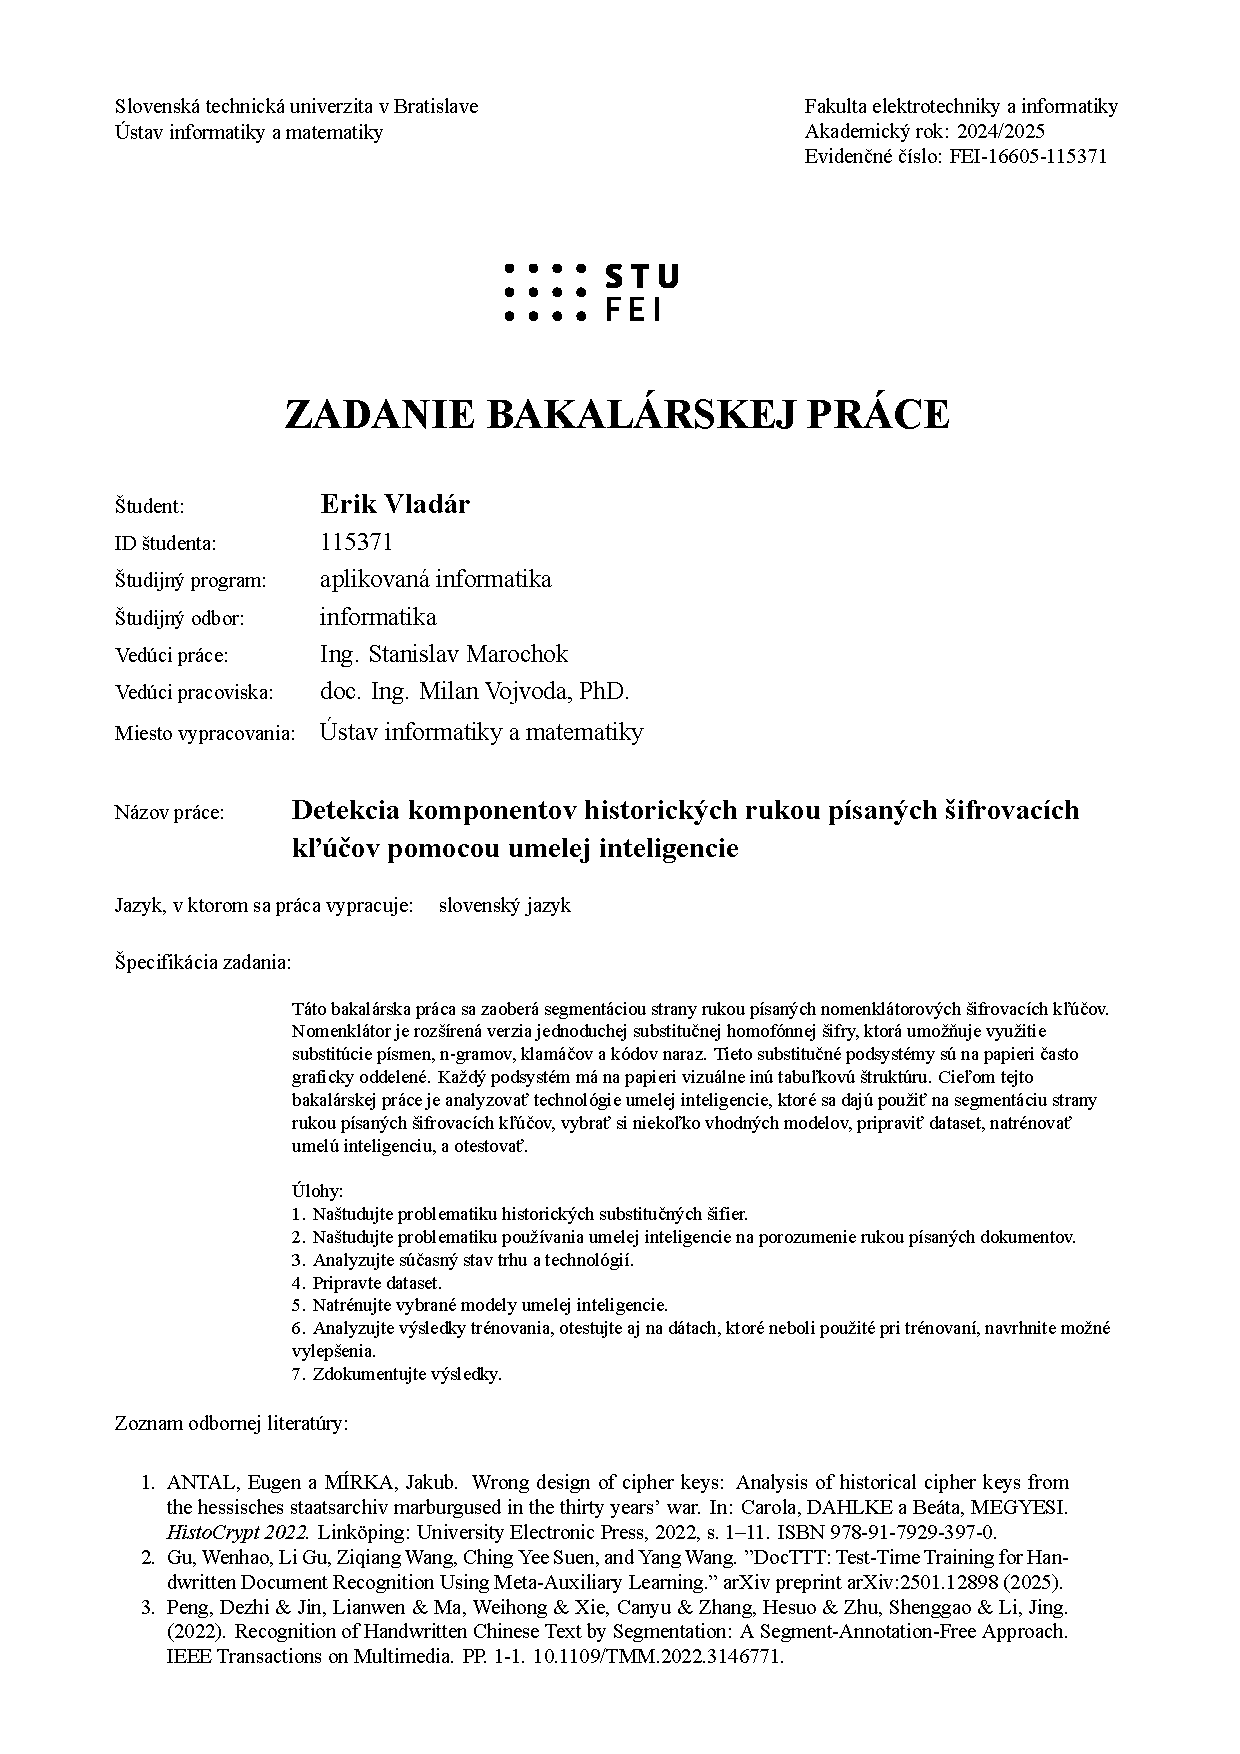
\includepdf[pages=-]{includes/file-10.pdf}
\FEIabstract{includes/abstract}
\FEIthanks{includes/thanks}
\FEIcontent
\FEIlistOfFiguresAndTables
\FEIlistOfListings

\mainmatter

\FEIintroduction{includes/introduction}
\FEIcore{includes/core}
\FEIconclusion{includes/conclusion}

\FEIbibliography %includes/bibliography.bib

\backmatter

\FEIlistOfAppendix
\FEIappendix{Použitie umelej inteligencie}{includes/AI_disclaimer}
\FEIappendix{Ukážka datasetu}{includes/dataset}
\FEIappendix{{Detailnejšie grafy alebo tabuľky}}{includes/graphs}
\FEIappendix{Dôležité časti kódu}{includes/codes}
\FEIappendix{Technická príručka}{includes/techHelp}

\end{document}
